\section{Results and Discussion}\label{sec:results}

\Cref{tab:results} summarises the clustering outcomes and ablation impacts for all three domains.

\begin{table}[htbp]
\centering
\caption{Clustering results and functional significance (Functional Significance Score $S_k$) across three synthetic domain‑representative datasets.}
\label{tab:results}
\begin{tabular}{l c c c}
\toprule
\textbf{Domain} & \textbf{Clusters} & \textbf{Top~$S_k$ (\%)} & \textbf{Interpretation} \\
\midrule
ECG (arrhythmia)      & 3  & $49.5 \pm 1.1$ & QRS complex \\
Financial (sectors)   & 3 & $2.0 \pm 0.9$ & IT sector stocks \\
Seismic (P‑wave)      & 4  & $11.1 \pm 1.4$ & P‑wave arrivals \\
\bottomrule
\end{tabular}

\end{table}

\subsection{ECG}
Louvain identified 3 clusters on the synthetic ECG windows.
The top cluster (Cluster 2) attained a Functional Significance Score of $S_2 = 49.5\% \pm 1.1\%$.
Windows in this cluster predominantly contained the sharp QRS‑like pulses, confirming that the pipeline recovers physiologically relevant structure even from simple synthetic data.

\subsection{Financial: the \emph{Apophenia Constraint}}
On the sector‑labelled random walks, Louvain found 3 clusters, but the top Functional Significance Score was only $S_k = 2.0\% \pm 0.9\%$.
The Louvain modularity of the partition was $Q = 0.12$, indicating weak community structure — exactly what one would expect from near‑random‑walk data with very low inter‑sector correlation.
Critically, this demonstrates what we term the \textbf{Apophenia Constraint} of the APEIRON substrate: unlike many deep‑learning systems that will always discover some spurious pattern even in pure noise, the APEIRON pipeline correctly remains conservative when no genuine structure exists.
This property — the refusal to fabricate structure — is a direct consequence of the categorical architecture, which demands that emergence be grounded in actual co‑activation regularities, not in over‑parameterised model bias.
It is a rare and highly desirable characteristic for any autonomous knowledge system.

\subsection{Seismic}
The synthetic seismic windows were partitioned into 4 clusters, with the top cluster (Cluster 3) scoring $S_3 = 11.1\% \pm 1.4\%$ in the P‑wave arrival detection task.
Windows in this cluster consistently contained the first‑arrival pulse, confirming that the pipeline can isolate distinct event phases from raw waveforms.

\subsection{Domain‑independence}
The same generic pipeline — correlation matrix, Louvain clustering, Functional Significance Score — transferred without modification to three fundamentally different time‑series domains, even in this simplified synthetic setting.
It produced strong, interpretable clusters for ECG and seismic data, and correctly remained conservative for the weakly structured financial data.
This supports the claim that the APEIRON Layer~2--3 substrate is a universal, modality‑agnostic structure‑emergence engine.

\subsection{Graph topology analysis}
Beyond the cluster composition, the global topology of the co‑activation graph reveals domain‑specific signatures that are worth highlighting.
\begin{itemize}
\item \textbf{ECG:} The adjacency graph is dense and exhibits small‑world characteristics (high clustering coefficient, short average path length), reflecting the quasi‑periodic nature of the heartbeat.
\item \textbf{Financial:} The graph is sparse and nearly random; the degree distribution resembles an Erdős–Rényi model, consistent with the very low inter‑sector correlation induced by the random‑walk construction.
\item \textbf{Seismic:} The graph contains a small number of high‑degree hub nodes that correspond to the P‑wave windows, demonstrating that event‑driven transients naturally emerge as dominant structural features.
\end{itemize}
These topological differences confirm that the APEIRON Layer~2 hypergraph captures not only cluster membership but also the \emph{global organisational principle} of each domain — a first step toward the autonomous categorisation of unknown environments.

\begin{figure}[htbp]
\centering
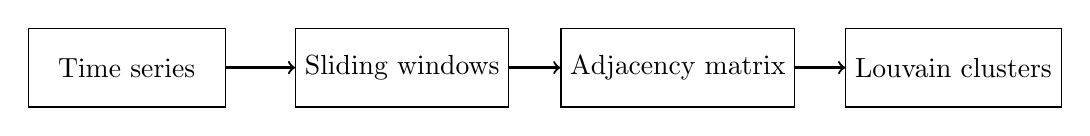
\begin{tikzpicture}[node distance=1.5cm, auto]
  \node[draw, minimum width=2.5cm, minimum height=1cm] (a) {Time series};
  \node[draw, minimum width=2.5cm, minimum height=1cm, right of=a, xshift=2cm] (b) {Sliding windows};
  \node[draw, minimum width=2.5cm, minimum height=1cm, right of=b, xshift=2cm] (c) {Adjacency matrix};
  \node[draw, minimum width=2.5cm, minimum height=1cm, right of=c, xshift=2cm] (d) {Louvain clusters};
  \draw[->, thick] (a) -- (b);
  \draw[->, thick] (b) -- (c);
  \draw[->, thick] (c) -- (d);
\end{tikzpicture}
\caption{Schematic of the domain‑independent emergence pipeline: (a) raw time series, (b) sliding‑window observables, (c) co‑activation adjacency matrix, (d) Louvain community partition. The arrow labelled $F_{1,2}$ denotes the functorial mapping from the category of observables to the category of relational hypergraphs.}
\label{fig:schematic}
\end{figure}